\documentclass[11pt,letterpaper]{article}

\usepackage[utf8]{inputenc}
\usepackage[T1]{fontenc}
\usepackage[spanish]{babel}
\usepackage{geometry}
\usepackage{xcolor}
\usepackage{graphicx}
\usepackage{hyperref}
\usepackage{array}

\geometry{margin=0.75in}
\definecolor{LynjaxNavy}{HTML}{083B5C}
\definecolor{LynjaxBlue}{HTML}{0E7490}
\definecolor{LynjaxTeal}{HTML}{2DD4BF}
\definecolor{LynjaxIce}{HTML}{F2FAF8}
\definecolor{LynjaxSlate}{HTML}{0F172A}

\hypersetup{
  colorlinks=true,
  linkcolor=LynjaxBlue,
  urlcolor=LynjaxBlue,
  pdftitle={Lynjax Beta 0.5 - Manual con Capturas Virtuales},
  pdfauthor={Lynjax / Alejandro Castillo}
}

\begin{document}

\begin{titlepage}
  \centering
  \vspace*{1.0cm}
  {\Huge\bfseries\color{LynjaxNavy} Lynjax Beta 0.5\\[0.25cm]}
  {\Large Intelligent Network Visibility\\[0.5cm]}
  {\Large Manual de prueba con capturas virtuales\\[1.0cm]}
  \rule{0.82\textwidth}{1pt}\\[0.5cm]
  {\large Backend FastAPI, Frontend React/Vite, lab local seguro y ruta de virtualización.\\[0.75cm]}
  {\large Fecha: \today\\}
  \vfill
  \begin{minipage}{0.82\textwidth}
  \textbf{Criterio operativo acordado:} los ambientes de prueba deben ejecutarse de forma virtualizada o sandboxed. No se debe tratar Windows local como runtime principal del lab. La virtualización por Intel Virtualization Technology fue confirmada desde BIOS, aunque algunos probes de sistema puedan reportar estados incompletos desde Git Bash/Windows.
  \end{minipage}
\end{titlepage}

\tableofcontents
\newpage

\section{Resumen ejecutivo}

Lynjax beta 0.5 es una base técnica para auditar, visualizar y documentar assessments de red con trazabilidad. Esta versión contiene:

\begin{itemize}
  \item Backend FastAPI con endpoints de health, metadata y assessment simulado.
  \item Frontend React/Vite con dashboard visual de assessment, evidencia y reporte.
  \item Lab Docker Compose local para targets HTTP sanitizados.
  \item Manuales Markdown y esta versión LaTeX/PDF con capturas virtuales.
  \item Scripts de arranque, parada, smoke tests y probe read-only del host.
\end{itemize}

\section{Política de virtualización y seguridad}

Para evitar contaminar el host Windows y mantener pruebas reproducibles:

\begin{itemize}
  \item Windows funciona como estación de control, no como runtime definitivo del lab.
  \item El runtime preferido para Docker/Compose es WSL2 Ubuntu/Debian o una VM Ubuntu con snapshot.
  \item No se deben tocar redes reales ni clientes sin autorización explícita.
  \item Los targets demo se limitan a loopback: \texttt{127.0.0.1}.
  \item El endpoint actual de assessment es simulado y declara \texttt{network\_access: disabled}.
\end{itemize}

\section{Estructura del proyecto}

\begin{tabular}{>{\bfseries}p{0.25\textwidth}p{0.68\textwidth}}
\texttt{backend/} & API FastAPI, schemas, servicios simulados y tests de contrato.\\
\texttt{frontend/} & Dashboard React/Vite con identidad visual Lynjax.\\
\texttt{lab/} & Fixtures y targets locales seguros para pruebas repetibles.\\
\texttt{virtualization/} & Compose beta y wrapper para ejecutar app + lab en runtime Docker/Linux.\\
\texttt{docs/} & Manuales Markdown, estado de beta y páginas auxiliares de captura.\\
\texttt{docs/manual/} & Fuente LaTeX, PDF y capturas virtuales de frontend/backend.\\
\texttt{reports/} & Plantilla inicial de reporte técnico de assessment.\\
\texttt{scripts/} & Automatizaciones de dev, smoke, lab y probe del host.\\
\end{tabular}

\section{Captura virtual del frontend}

La Figura~\ref{fig:frontend} muestra el dashboard visual de Lynjax. La captura fue generada desde una sesión de navegador automatizada sobre el build del frontend y almacenada dentro del proyecto en \texttt{docs/manual/assets/screenshots/frontend-dashboard.png}.

\begin{figure}[htbp]
  \centering
  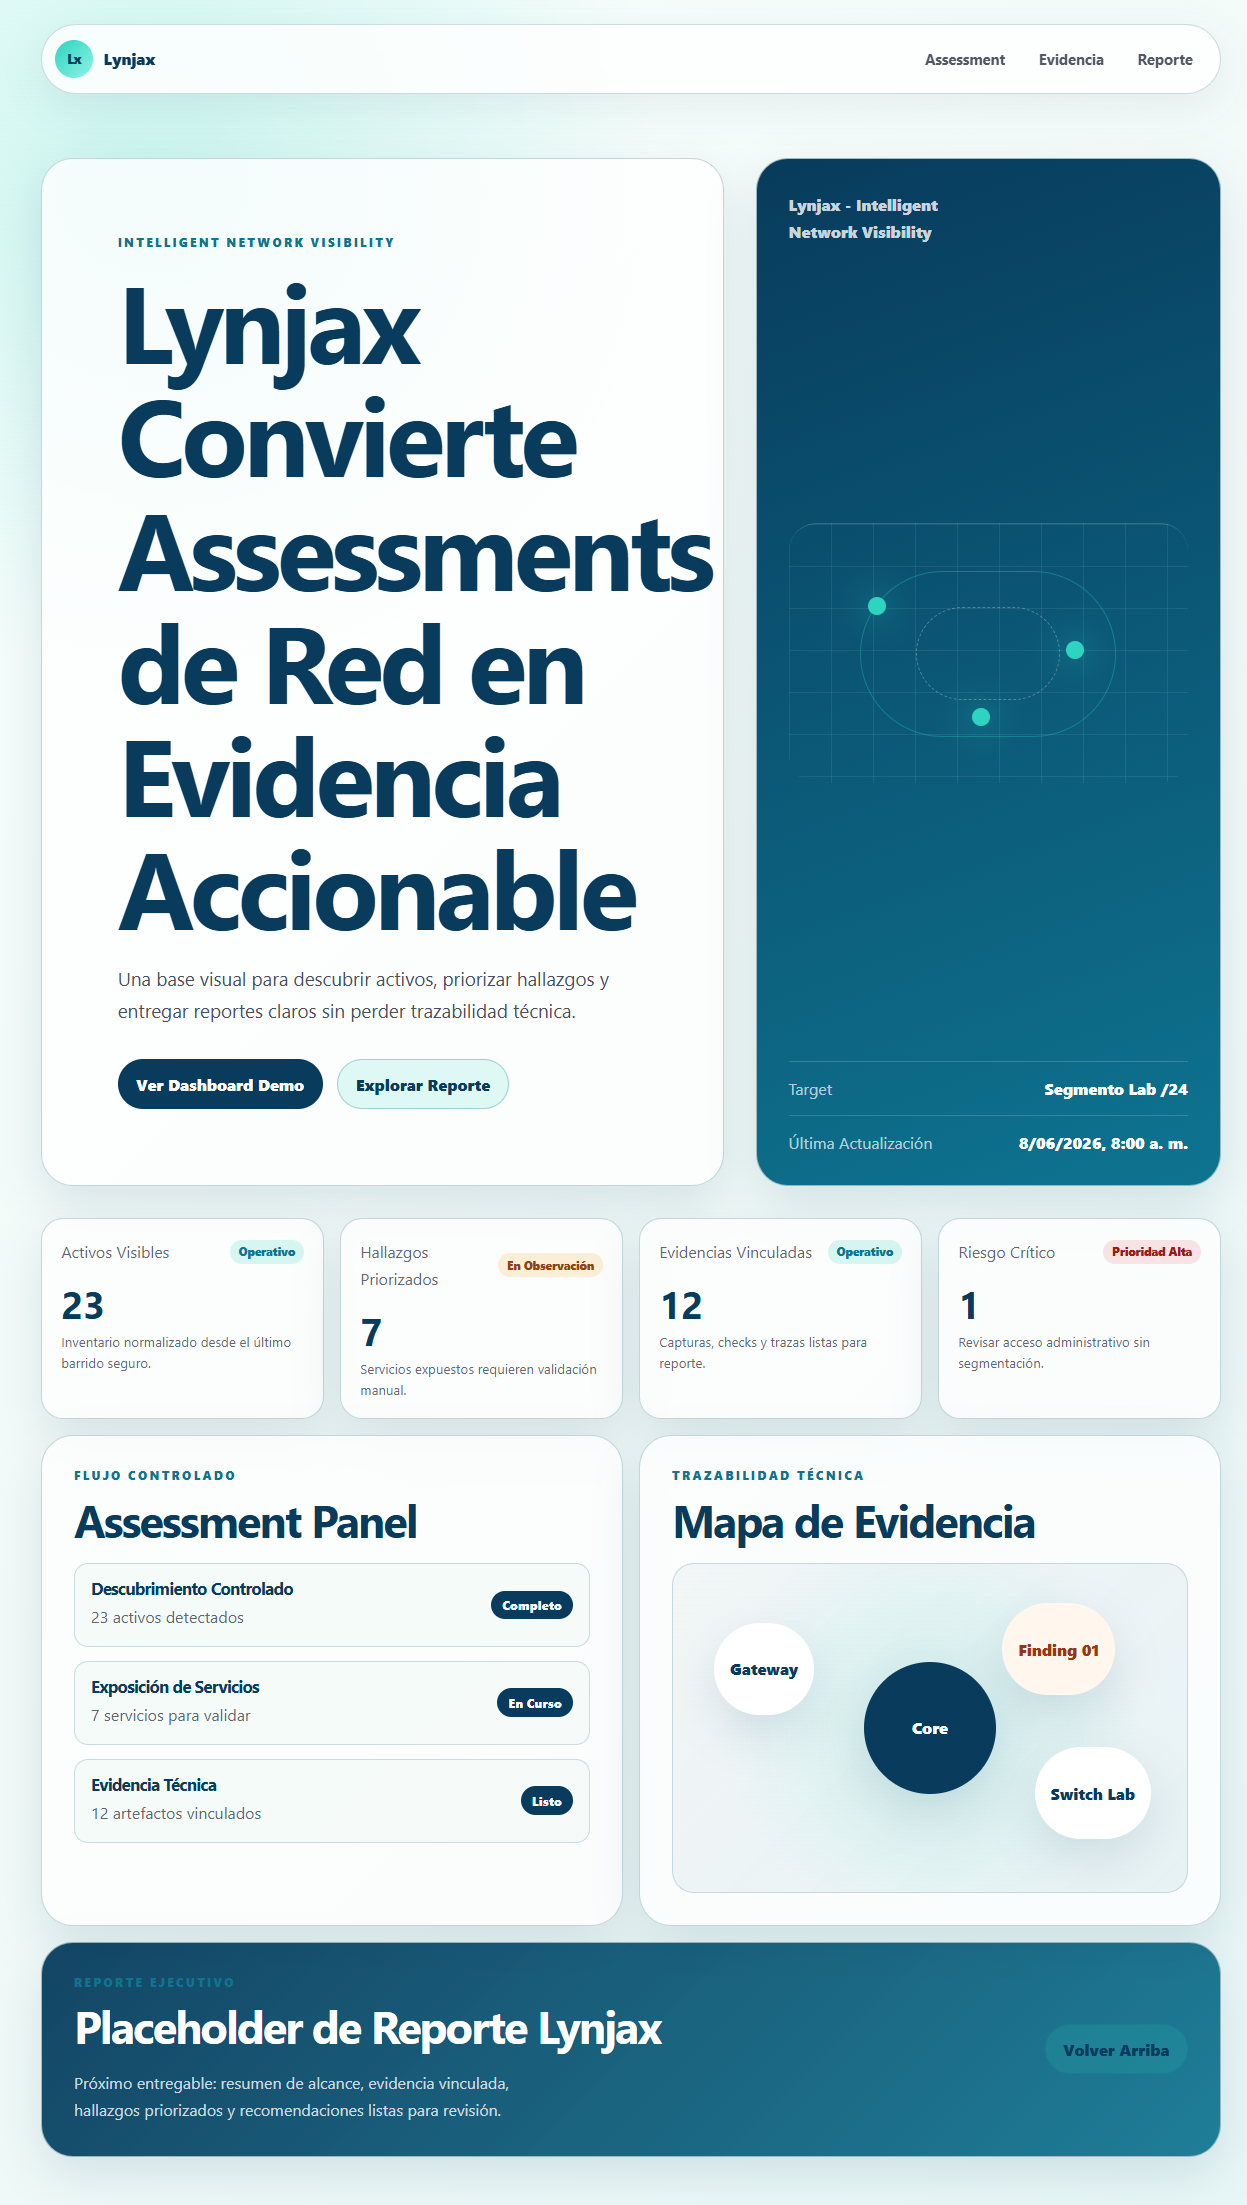
\includegraphics[width=0.98\textwidth,height=0.82\textheight,keepaspectratio]{../assets/screenshots/frontend-dashboard.png}
  \caption{Dashboard frontend Lynjax con hero, métricas, panel de assessment, mapa de evidencia y placeholder de reporte.}
  \label{fig:frontend}
\end{figure}

\subsection{Funcionalidades visibles}

\begin{itemize}
  \item Navegación superior: Assessment, Evidencia y Reporte.
  \item Hero de producto con tagline \emph{Intelligent Network Visibility}.
  \item Tarjetas de estado: activos visibles, hallazgos priorizados, evidencias y riesgo crítico.
  \item Panel de flujo controlado para checks de assessment.
  \item Mapa visual de evidencia con nodos de red y hallazgo.
  \item Sección de reporte ejecutivo como siguiente entregable.
\end{itemize}

\section{Captura virtual del backend}

La Figura~\ref{fig:backend} documenta la vista de backend preparada para manuales. Resume contratos API y una respuesta demo generada desde el backend FastAPI mediante cliente de pruebas, sin ejecutar probes contra redes reales.

\begin{figure}[htbp]
  \centering
  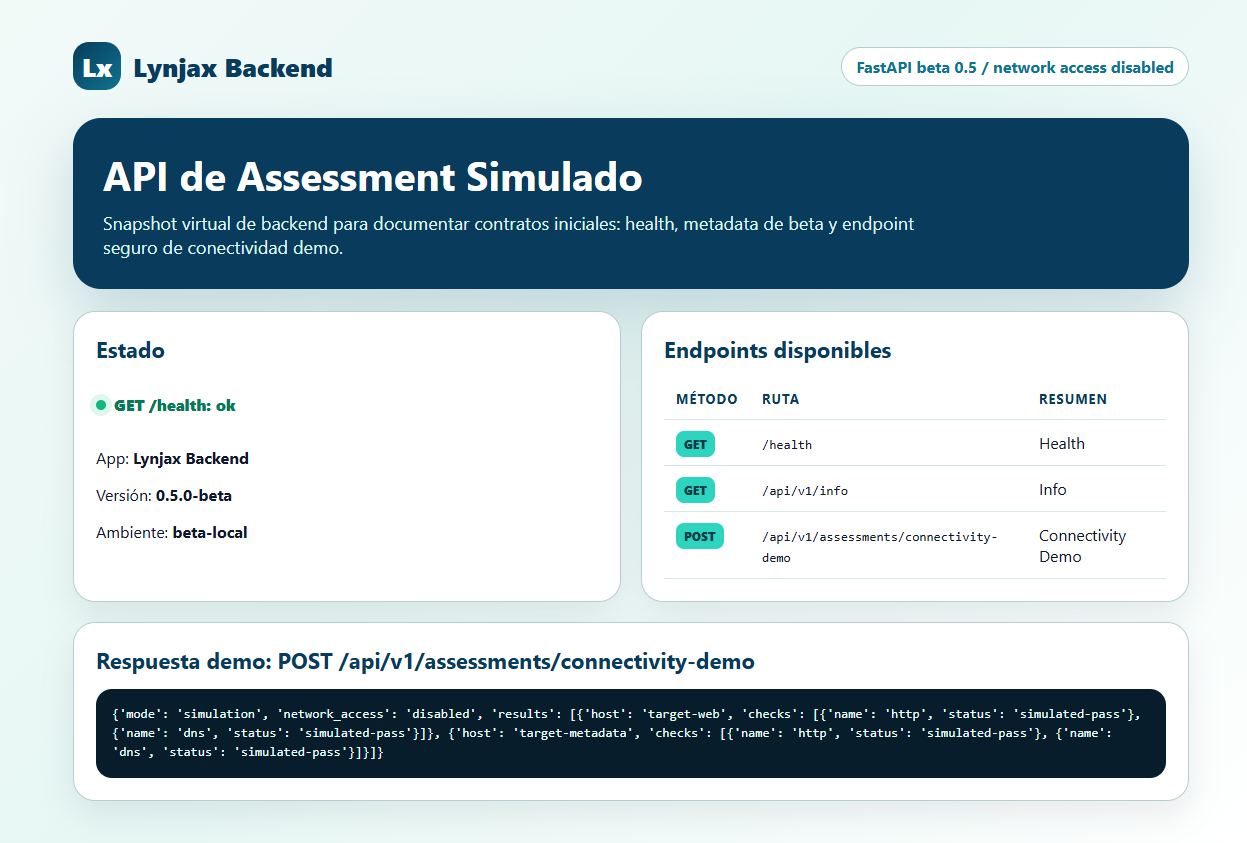
\includegraphics[width=0.98\textwidth,height=0.78\textheight,keepaspectratio]{../assets/screenshots/backend-api.png}
  \caption{Snapshot virtual del backend Lynjax: health, endpoints disponibles y respuesta simulada de connectivity-demo.}
  \label{fig:backend}
\end{figure}

\subsection{Contratos iniciales del backend}

\begin{itemize}
  \item \texttt{GET /health}: verifica disponibilidad básica de la API.
  \item \texttt{GET /api/v1/info}: expone metadata de beta, versión, entorno y política de red.
  \item \texttt{POST /api/v1/assessments/connectivity-demo}: devuelve resultados simulados por host/check.
\end{itemize}

\section{Comandos de prueba}

\subsection{Validación local controlada}

Estos comandos validan artefactos del repo. Para el lab completo, ejecutar preferiblemente dentro de WSL2/VM/CI.

\begin{verbatim}
python -m pytest backend/tests -v
npm --prefix frontend run build
bash scripts/lab_validate.sh
\end{verbatim}

\subsection{Arranque de demo frontend/backend}

\begin{verbatim}
bash scripts/dev-start.sh
bash scripts/smoke-local.sh
bash scripts/dev-stop.sh
\end{verbatim}

\subsection{Virtualización beta}

\begin{verbatim}
bash scripts/host-probe.sh
cd virtualization
bash run-beta-compose.sh config
bash run-beta-compose.sh up
bash run-beta-compose.sh down
\end{verbatim}

\section{Criterios de aceptación}

\begin{itemize}
  \item Backend tests pasan: \texttt{3 passed}.
  \item Frontend compila con Vite sin errores.
  \item Las capturas virtuales existen en \texttt{docs/manual/assets/screenshots/}.
  \item El PDF se genera en \texttt{docs/manual/lynjax-beta-0.5-manual.pdf}.
  \item El lab Compose se valida en WSL2/VM/CI cuando Docker esté disponible.
\end{itemize}

\section{Próximos pasos}

\begin{enumerate}
  \item Conectar el frontend al endpoint real \texttt{/api/v1/assessments/connectivity-demo}.
  \item Generar reportes Markdown/LaTeX/PDF desde datos devueltos por la API.
  \item Añadir persistencia local mínima para ejecuciones y evidencias.
  \item Mantener los manuales en tres formatos: Markdown, LaTeX y PDF.
  \item Incluir capturas virtuales actualizadas en cada entrega funcional.
\end{enumerate}

\end{document}
